\documentclass[11pt]{article}
\usepackage[utf8]{inputenc} % Para caracteres en espa�ol
\usepackage{amsmath,amsthm,amsfonts,amssymb,amscd}
\usepackage{multirow,booktabs}
\usepackage[table]{xcolor}
\usepackage{fullpage}
\usepackage{lastpage}
\usepackage{enumitem}
\usepackage{multicol}
\usepackage{fancyhdr}
\usepackage{mathrsfs}
\usepackage{wrapfig}
\usepackage{setspace}
\usepackage{esvect}
\usepackage{calc}
\usepackage{multicol}
\usepackage{cancel}
\usepackage{graphicx}
\graphicspath{ {pictures/} }
\usepackage[retainorgcmds]{IEEEtrantools}
\usepackage[margin=3cm]{geometry}
\usepackage{amsmath}
\newlength{\tabcont}
\setlength{\parindent}{0.0in}
\setlength{\parskip}{0.05in}
\usepackage{empheq}
\usepackage{framed}
\usepackage{newtxmath}
\usepackage{euscript}
\DeclareMathAlphabet{\mathpzc}{T1}{pzc}{m}{it}
\usepackage[most]{tcolorbox}
\usepackage{xcolor}
\colorlet{shadecolor}{orange!15}
\parindent 0in
\parskip 12pt
\geometry{margin=1in, headsep=0.25in}
\theoremstyle{definition}
\newtheorem{defn}{Definition}
\newtheorem{reg}{Rule}
\newtheorem{exer}{Exercise}
\newtheorem{note}{Note}
\newcommand{\volume}{{\ooalign{\hfil$V$\hfil\cr\kern0.08em--\hfil\cr}}}
\newcommand{\parr}{\mathbin{\|}} % Parralel Symbol
\begin{document}
\setcounter{section}{1} %Section before the section you want. I want section 1 I put 0
\setcounter{page}{9} %page number you want to be the first page
\setcounter{equation}{16} %equation before the equation you want I want equation 2 I put 1
%\definecolor{babyblue}{rgb}{0.54, 0.81, 0.94}
\definecolor{babyblueeyes}{rgb}{0.63, 0.79, 0.95}
\definecolor{babyblue}{rgb}{0.69, 0.88, 0.9}

 \pagestyle{fancy}
 
\fancyhf{}
\rhead{Section 5:  Collisions}
\rfoot{Page \thepage}
\thispagestyle{empty}


\begin{center}
{\LARGE \bf Section 5:  Collisions}\\
{\large AE435}\\
Spring 2018
\end{center}
\vspace{5mm}
\section{Electron-Atom Collisions}
\vspace{25mm}
\tableofcontents
\newpage
\subsection{Elastic} 
There is a severe energy dependence for each species, and little resemblance between species.  Recall previously in which we discussed the resonance of orbit radius with electron wavelength. The resulting effect (Ramsauer effect) causes dramatic dips in Fig 4-3. In this figure, the y-axis is the total or effective cross section and the x-axis the is energy of the particles in eV. 
\newline
\begin{center}
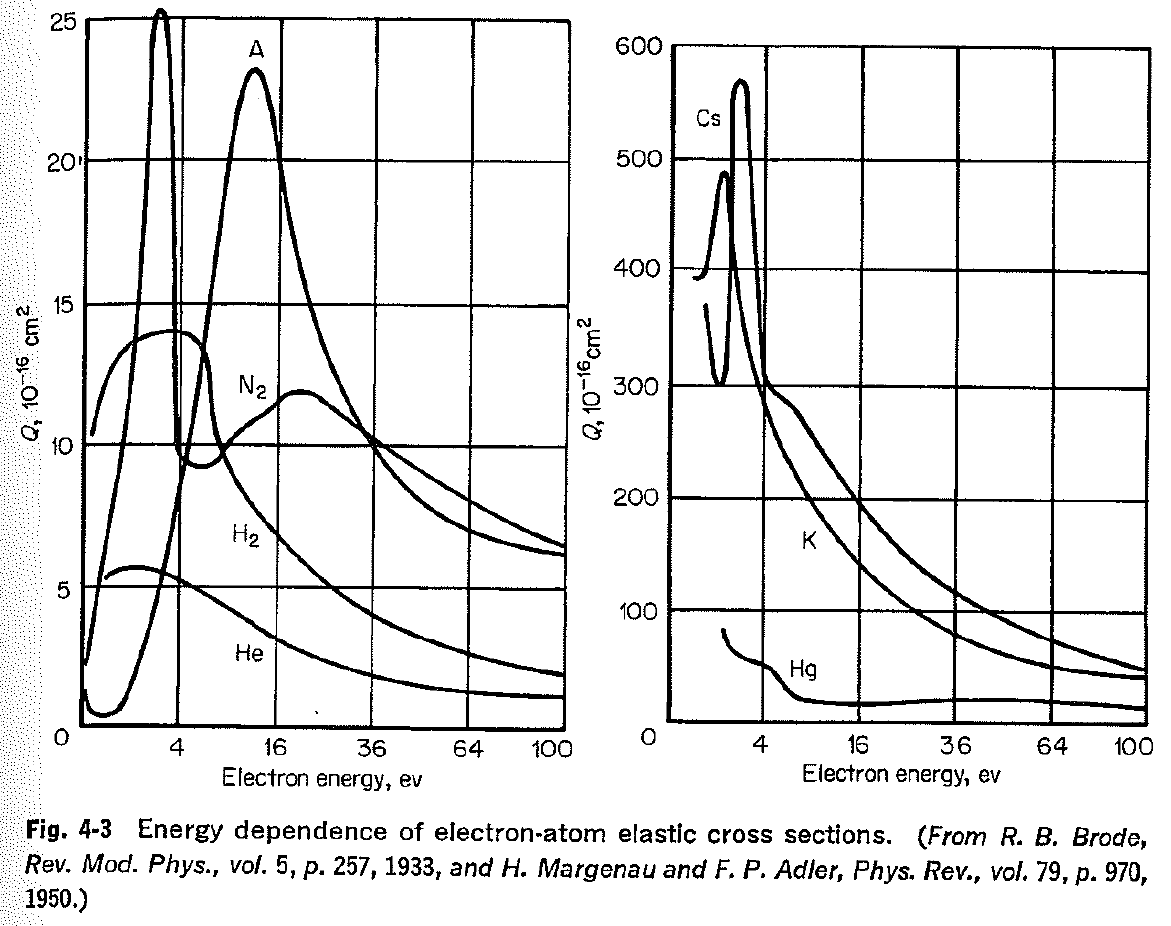
\includegraphics[scale=.55]{2.png}
\end{center}
\newpage
In Figure 4-4 below, we now see a severe angular dependence.  A vastly different results from our previous, constant-diameter billiard ball model. In Figure 4-4, the y-axis is the differential cross section and the x-axis is the scattering angle, $\theta$.

\begin{center}
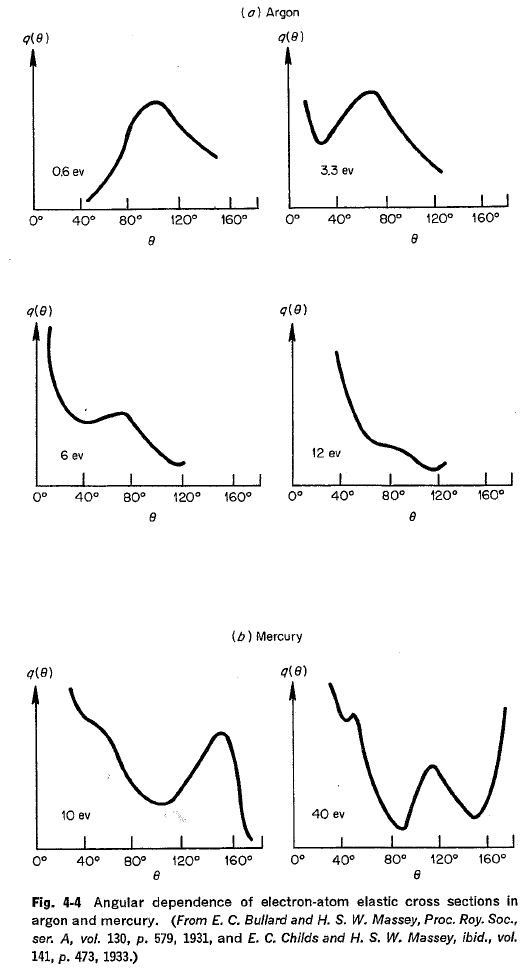
\includegraphics[scale=.7]{3.png}
\end{center}

We observe that in the 3.3eV case for Argon atoms, the most preferred scattering angle is $\theta = 75^{\circ}$. Though Argon was the propellant gas of choice when the Jahn textbook was released, modern day electric propulsion systems use Xenon.
\newpage
Given that modern day electric propulsion systems use a Xenon propellant, the following experimental data is used. Here we see electrical scattering from differential cross-sections. Take note that the units for the differential cross-section here are $a_o^2 \, sr^{-1}$.
\begin{center}
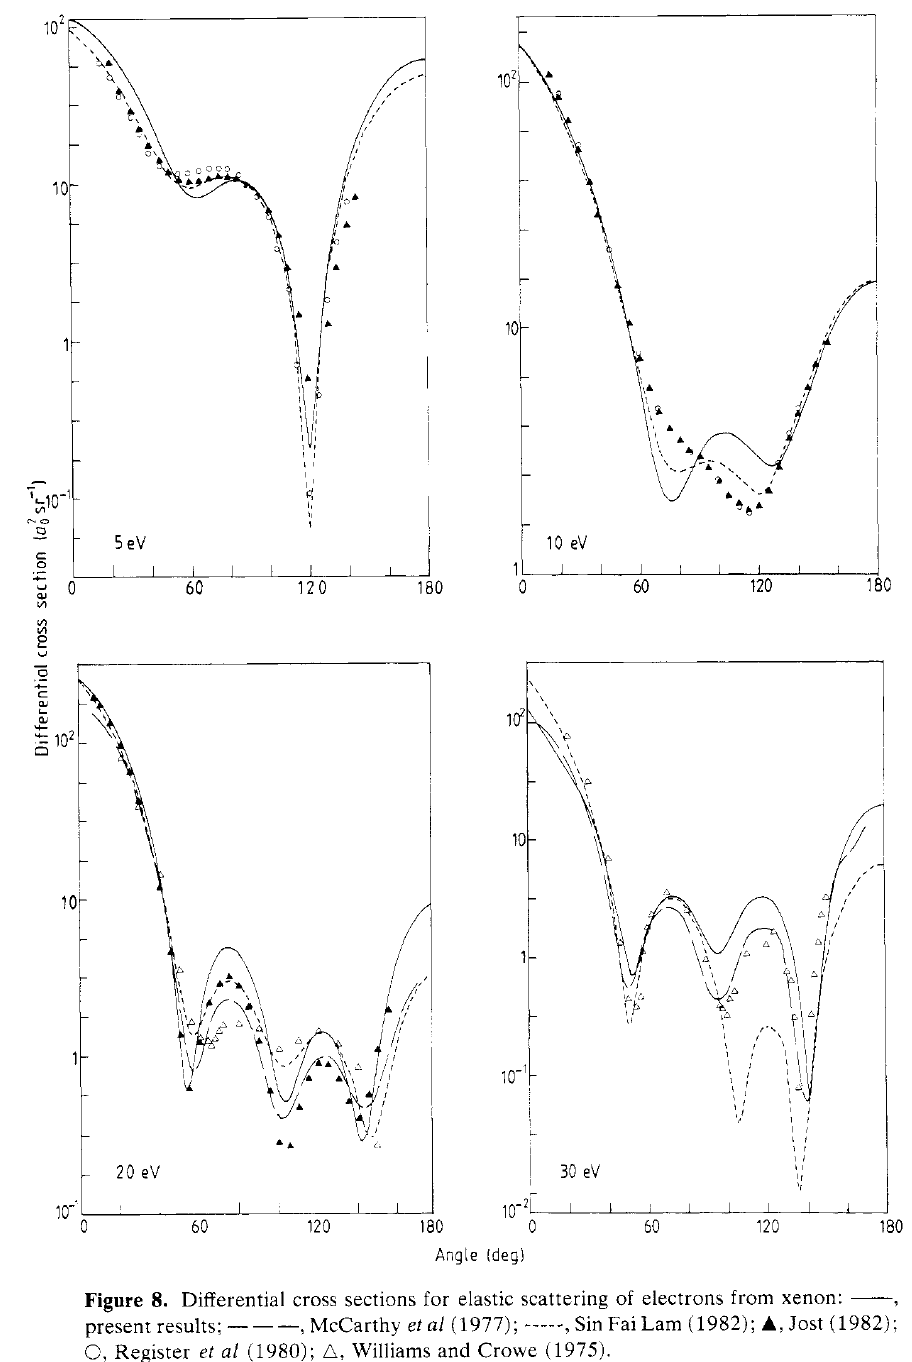
\includegraphics[scale=.55]{4.png}
\end{center}
\newpage
Finally, we have the plot for total scattering cross-section for electrons of Xenon.
\begin{center}
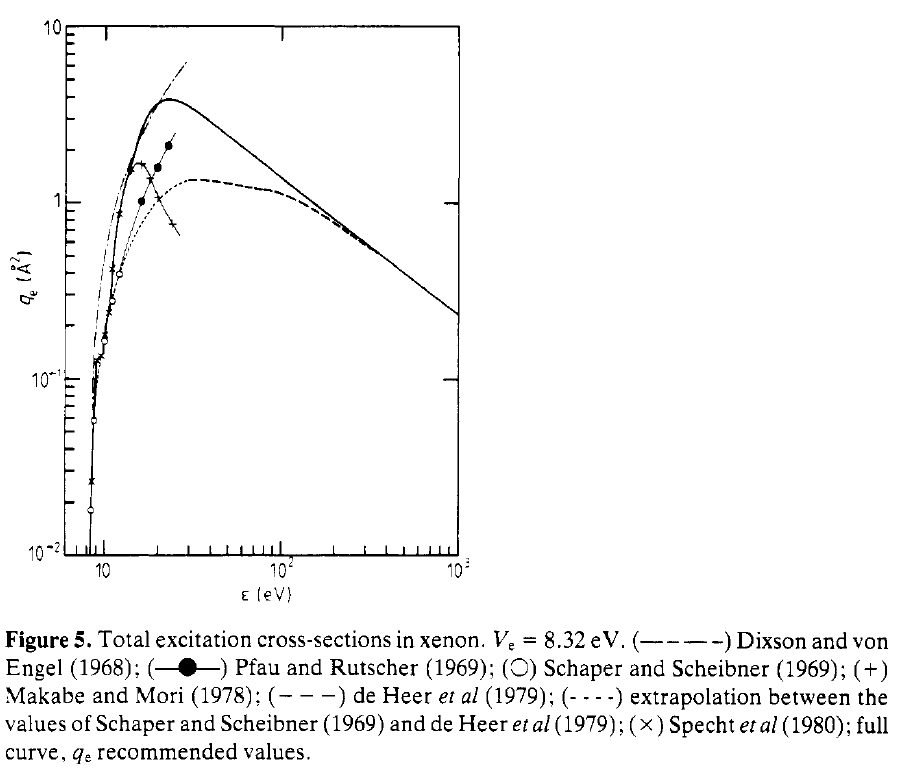
\includegraphics[scale=.7]{7.png}
\end{center}
\newpage

\subsection{Inelastic}
Inelastic collisions are the most important reactions for electric propulsion systems. These collisions include

 \textbf{Excitation (Bound-Bound Transition):} An electron orbiting an atom has been bumped up into a higher orbital.
 \begin{equation*}
 \begin{aligned}
 \tilde{e} + A \rightarrow A^* + e
 \end{aligned}
 \end{equation*}
And 

\textbf{Ionization (bound-free transition)}
  \begin{equation*}
 \begin{aligned}
  \tilde{e} + A \rightarrow A^+ + 2e
 \end{aligned}
 \end{equation*}
 
Both reactions require a certain threshold amount of energy, called the excitation potential         $\varepsilon_{ex}$  	or ionization potential     $\varepsilon_i$     	.  In the above,
\begin{itemize}
   \item 	$\tilde{e} \, \,$ : An electron with energy greater or equal to the excitation or ionization potential
   \item 	$A^*$ : An excited atom (bound electron boosted to higher-energy orbit)
   \item 	$A^+$ : An ion (bound electron ejected from valence shell)
 \end{itemize}
\newpage
Typical excitation cross-sections for helium
%Helium isnt used as much anymore...notice the cross section drops below 0 past the ionization threshold. If electrons dont have enough energy you cant excite the electrons.
\begin{center}
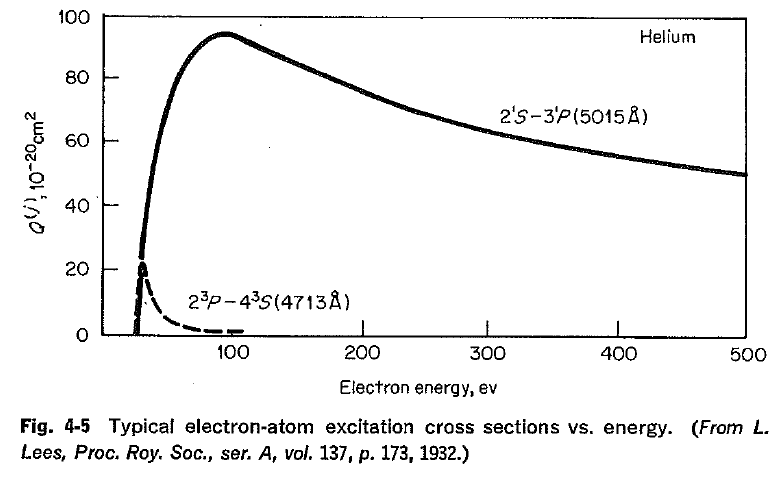
\includegraphics[scale=.7]{6.png}
\end{center}
From Figure 4-5 we can see that the
 \begin{itemize}
\item "allowed" transition (by quantum mechanics rules) is the upper line; falls as 	
\item "forbidden" transition is lower line;  fall as
\end{itemize}
Note that cross-section drops to zero below the ionization threshold, $\varepsilon_{th} = \varepsilon_{ex}$. This makes sense! If electrons do note have enough energy, they cannot get excited (simply conservation of energy, can't excite if impact energy is insufficient).
 \newpage
From the M Hayashi paper published in the Journal of Physics D: Applied Physics, Volume 16, Number 4, the figure below shows the excitation cross sections for Xenon.
 \begin{center}
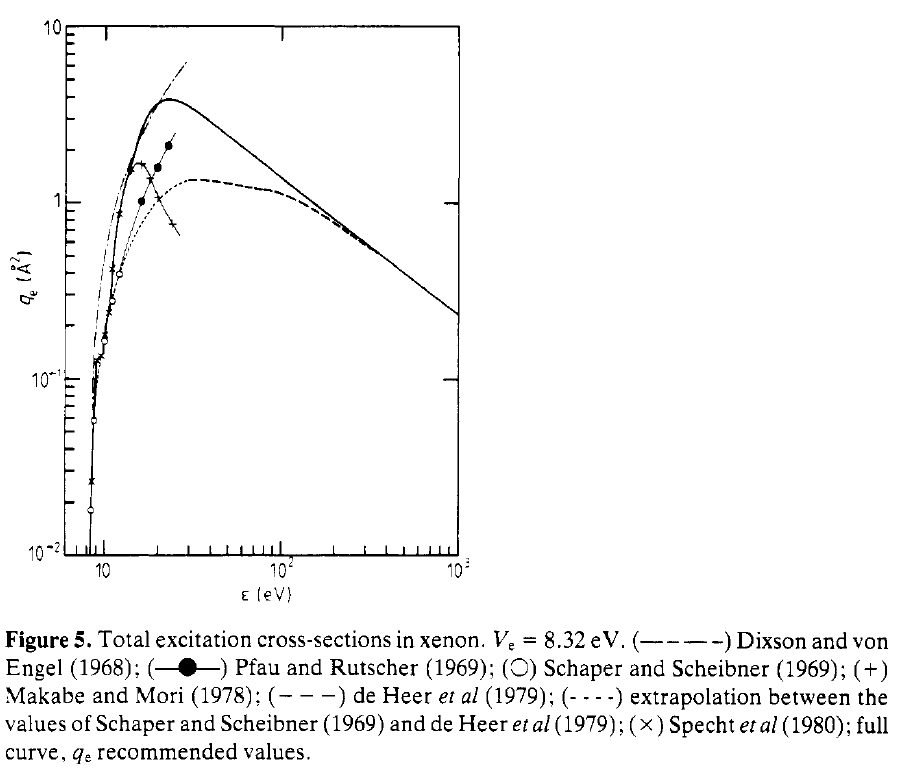
\includegraphics[scale=.7]{7.png}
\end{center}
 From this figure, we see that the total excitation cross-sections in xenon, has an excitation threshold, $V_e = 8.32 \, eV$.
 \newpage
Typical ionization cross-sections for Hydrogen (monatomic and diatomic). Note that Hydrogen is still fairly common in electric propulsion systems, especially in arcjets / resistojets
 \begin{center}
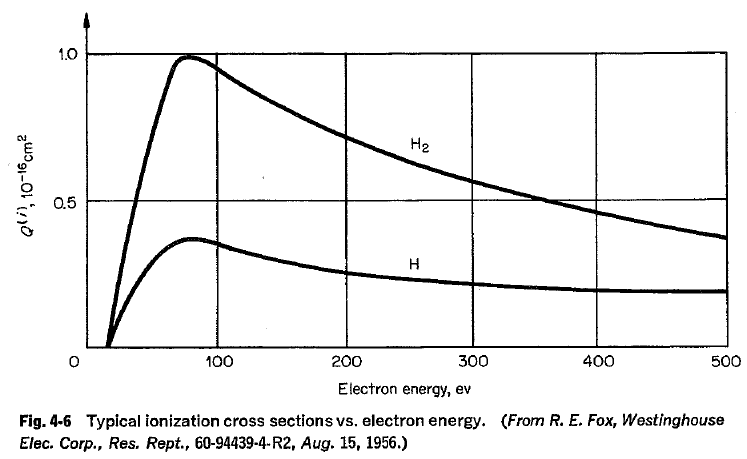
\includegraphics[scale=.8]{8.png}
\end{center}
In this figure... 
\begin{itemize}
\item Molecular hydrogen (upper line)
\item Atomic hydrogen (lower line)
 \end{itemize}
 \newpage
 
This figure shows the ionization cross section vs. the electron energy. 
 \begin{center}
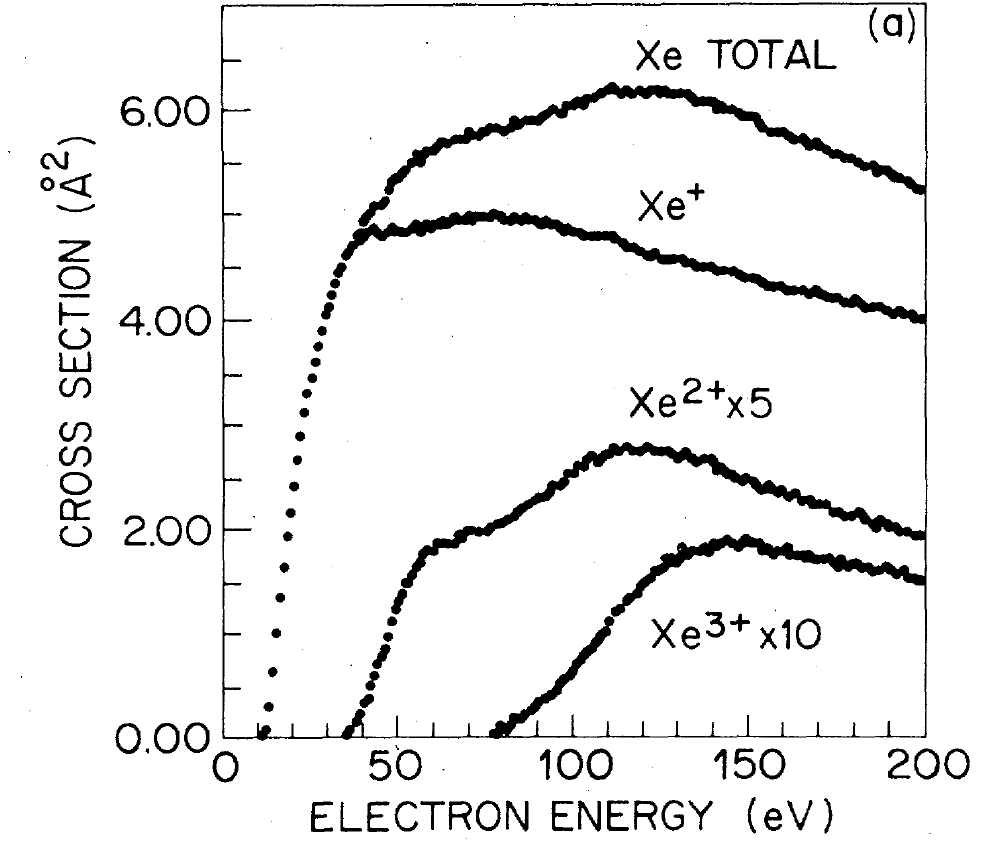
\includegraphics[scale=.45]{9.png}
\end{center}
As we can see, the ionization threshold for xenon is $\varepsilon_{iz,xe} = 12.13 \, eV$. Showing collision cross sections between electrons and Xenon atoms. In these plots, the $\times 5$ means these cross sections have been multiplied by 5. This was done so it all can show up on the same plot.

Calculating the excitation and ionization rates:  mean electron speed is almost always much higher than mean neutral speed.
  \begin{equation*}
 \begin{aligned}
\vv{v}_e >> \vv{v}_A
 \end{aligned}
 \end{equation*}
 The velocity of electrons is always much much higher than the velocity of atoms.
 %velocity of electrons always muc much higher than that of atoms

The collision rate in a gas with number density $n_a$, is
  \begin{equation}
 \begin{aligned}
 n_a \, \nu_{ae}^i = n_a \int n_e \, (\vv{v}_e)\, Q_{ae}^i \, (\vv{v}_e) \, \vv{v}_e \, \mathrm{d}v_e
 \end{aligned}
 \end{equation}
Superscript stands for ionization or excitation. This came from equation16
 
 \newpage
We can make some assumption in Equation 17. Looking at the figure below, we see that the plot on the left is the energy distribution function for the electrons of the gas/plasma. The right curve is the cross section as a function of the energy. We can look at the two curves and plot them on same x-axis. 

\textbf{Question: }What can we tell about the electrons? Which of the electrons in the distribution can do the ionization or excitation?

\textbf{Answer: } Answer: The electrons in the tail do. The electrons on the tail are doing the excitation and ionization. 

Another thing we can do with the Equation 17 is approximate Q (the cross section) as just a straight lines. If we consider the cross section to be linear in the lower energy end.
 \begin{center}
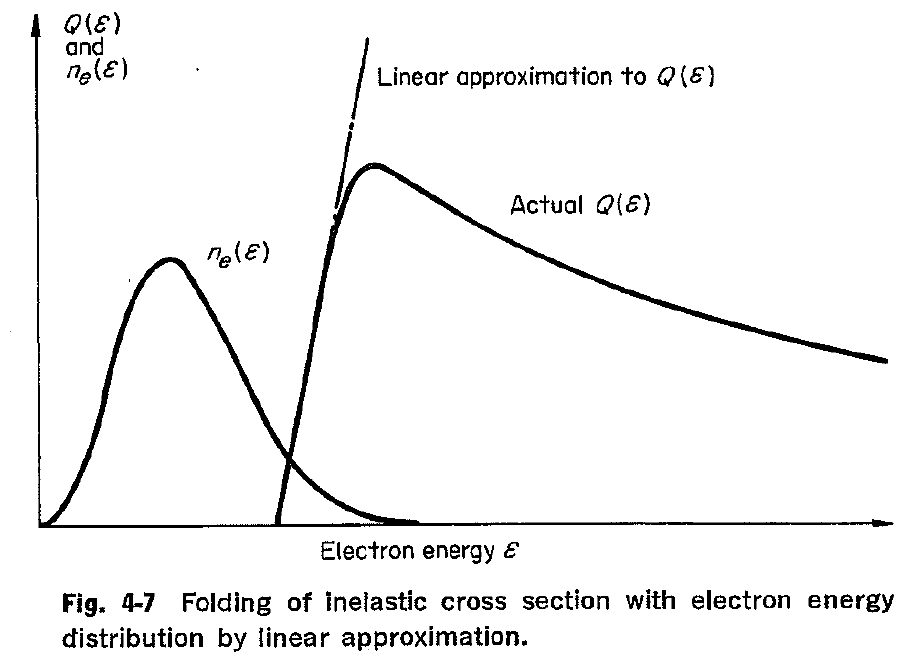
\includegraphics[scale=.55]{10.png}
\end{center}
 Figure 4-7 shows
  \begin{itemize}
\item typical cross section Q, is a function of energy ($Q(\varepsilon)$) where $\varepsilon = \frac{1}{2} \, m \, v_e^2$
\item Electron energy distribution function,   $n_e \, (\vv{v}_e)$       (e.g., might be Maxwellian)
\item EEDF tails off around the peak of  Q , you can make a linear approximation in the collision rate integral (5.17)
\item Also note, only the high-energy tail of the EEDF participates in these processes (e.g., excitation, ionization)
\end{itemize}
%excitation and ionization are the most importatnt for EP. Xenon is typical prop.
\end{document}